\documentclass{uva-inf-article}
\usepackage[english]{babel}
\usepackage{graphicx}
\usepackage{algorithm}
\usepackage{algorithmic}
\usepackage[document]{ragged2e}
\usepackage{blindtext}
\usepackage{enumitem}
\usepackage[style=authoryear-comp]{biblatex}
\addbibresource{references.bib}
\graphicspath{ {./images/} }


\title{Building a Manufacturing
Robot Software System}

\assignment{RWA67}
\assignmenttype{Report}

\authors{Shreejay Badshah, Arshad Shaik, Tej Kiran, Tim Sweeney, Dhinesh Rajasekaran, Ian Serbin}

\tutor{Dr. Zeid Kootbally \\Dr. Craig Schlenoff}
\group{Group 2}

\course{Summer2023}
\courseid{ENPM663}


\date{August, 2023}

\begin{document}
\maketitle 
\newpage
\tableofcontents
\newpage
\listoffigures
\newpage
\setlength{\hsize}{0.9\hsize}
\justifying
\section{Introduction}
This report summarizes the work done in RWA67 for Building a Manufacturing Robot Software
System (ENPM663). RWA67 comprises a Competitor Control System (CCS) that can handle insufficient part, and faulty part challenges in ARIAC competition.\\

\noindent ARIAC (Agile Robotics for Industrial Automation Competition) is hosted by NIST (National Institute of Standards and Technology) to test the agility of the industrial robot system. The purpose of ARIAC is to make industrial robots more autonomous, productive with minimum human input.\\

\noindent In this competition, several types of parts; sensors, pumps, regulators and batteries; in several colors; red, blue, green, orange and purple; are provided in a Gazebo simulation environment to complete orders. The order type can be for kitting, assembly, or kitting and assembly. At competition start, parts are introduced into the environment using a conveyor belt and then are placed on bins for the required orders. A floor robot is provided in the environment to pick parts from the conveyor belt and place them on bins. There 8 similar bins in the environment. After receiving all the parts and storing them on the bins, the floor robot then again picks these parts from the bins and places them on an automated guided vehicle (AGV) tray to fulfill required orders. The floor robot also has a gripper type that can pick and place trays on AGVs before putting parts on them. The fulfilled order is then submitted to the warehouse.  Once all orders have been kitted/assembled and shipped to the warehouse, the ARIAC competition is ended.  Competition score is computed and determined based on how successful the CCS was at filling orders and managing agility challenges.\\

\noindent Several challenges are introduced in the competition to test the agility of the competitor control system. These challenges are:\\

\begin{minipage}{13.5cm}
\begin{enumerate}
    
    \item \justifying Faulty Part 
    \item \justifying Insufficient Part 
    \item \justifying High Priority Order.
    \item \justifying Flipped Part \\
\end{enumerate}
\end{minipage}

\noindent The focus of this RWA is to address faulty part and insufficient part challenge to complete kitting orders.\\

\begin{figure}[h]
\centering
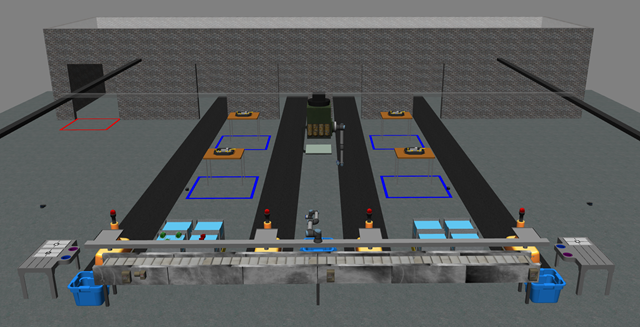
\includegraphics{images/ARIAC.png}
\caption{ARIAC Arena}
\label{fig:swArch}
\end{figure}

\justifying
\section{Problem Statement}
For this course the problem was to test the agility of an industrial floor robot to complete kitting tasks with the challenges of:\\

\begin{minipage}{13.5cm}
\begin{enumerate}
    \item \justifying Faulty part challenge:\\
    In this challenge a part placed on certain quadrant of a tray, placed on an AGV, can be deemed faulty. In case a faulty part is detected then CCS must discard this part in discard bin to avoid a penalty.
    \item \justifying Insufficient parts challenge:\\
    Sometimes in the competition there are not enough parts to fulfill an order. In this case the order still must be submitted with as many parts available as possible to avoid a penalty.
\end{enumerate}
\end{minipage}


\justifying
\section{Software Architecture}

The software architecture for the project implementation is depicted in Figure \ref{fig:swArch}.\\

\newline
\noindent \underline{Order Manager:}  The heart of the architecture is the 'order manager', which manages different services, manages communication with ARIAC, communicates with the motion planning node, etc. A detailed description of the 'order manager' is given in the subsequent corresponding section \ref{OrderManager} further down the document.\\

\newpage
\begin{figure}[h]
    \centering
    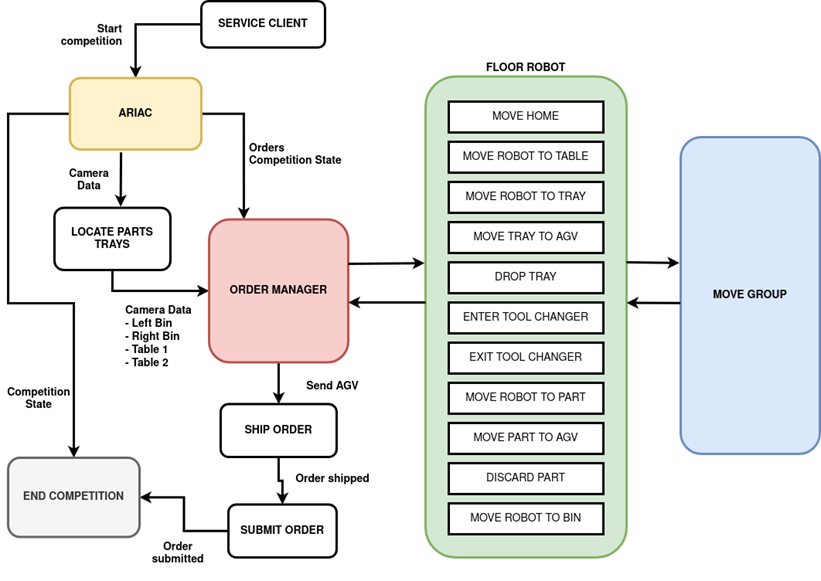
\includegraphics[scale=0.75]{images/SW_Architecture.png}
    \caption{Software Architecture}
    \label{fig:swArch}
\end{figure}
\noindent 

\noindent \underline{FLoor Robot: } The floor robot node's primary function is to communicate with move group node to generate a motion plan for the robot.  The floor robot instantiates services that allow for high level movements to be broken down into smaller movements and communicated with the Move Group.   Functionalities of each of the services are as described below:

\begin{itemize}
    \item Move Home:                      Moves the floor robot to the home position (center of the rail)

    \item Move Robot to Table:       Moves the robot to the specified tray table/gripper changer station

    \item Move Robot to Tray:         Moves the end effector of the robot to the specified tray

    \item Drop Tray:                          Drops the tray

    \item Enter Tool Changer:         Enter the specified tool changer (part or tray gripper) at the specified table

    \item Exit Tool Changer:            Exits the specified tool changer

    \item Move Robot to Part:         Moves the robots end effector to the specified part

    \item Move Part to AGV:            Once the part is picked up, move it to the specified AGV

    \item Discard Part:                      Drops the carried part

    \item Move Robot to Bin:           Moves the robot to the center trash bin 
\\
\end{itemize}

\noindent \underline{Locate Parts and Trays:}   Locates the part and tray locations/orientations, as determined by the camera sensors.\\

\noindent \underline{Service Client:}Begins the competition.\\

\noindent \underline{Ship Order:} Moves the specified AGV to the warehouse.\\

\noindent \underline{Submit Order:} Submits a transported order for grading.\\

\noindent \underline{End Competition:} Ends the competition.\\\\


\noindent Terminologies associated with the architecture are defined below:\\

\noindent \underline{Competitor Control System (CCS): }
The competitor control system (CCS) is the software that is provided by competitors. The CCS is responsible for communicating with the competition environment and executing the tasks.\\

\noindent \underline{Order: }
An order is an instruction containing information on a task ( Kitting Task, Assembly Task, or Combined Task,). Each task consists of at least one part of a specific color and type.\\

\noindent \underline{Part: }
Parts are used during pick-and-place operations. There are four available parts (battery, pump, regulator, and sensor) and each part can be one of five possible colors (red, green, blue, orange, and purple).\\

\noindent \underline{Trial: }
Each run of the competition is called a trial. The configuration for that trial is defined by a configuration file (YAML). Competitors do not and must not directly read trial files but needs to use topics and services provided by the competition environment.\\

\noindent \underline{Kitting Task: }
Kitting is the process which groups separate but related parts as one unit. For a kitting task, competitors are expected to:

-Place a kit tray onto one of the four AGVs.
-Place parts onto that kit tray in a specific quadrant.
-Direct the AGV to the warehouse.
-Evaluate the submitted kit for scoring.\\

\noindent \underline{Launch file Setup: }
A single ROS2 launch file is created that starts the competition and runs all the required packages/ nodes as shown below:\\
    -\verb|moveit|\\
    -\verb|included_launch|\\
    -\verb|service_client_exe_node|\\
    -\verb|locate_parts_trays_exe_node|\\
    -\verb|order_manager_node|\\
    -\verb|ship_order_exe_node|\\
    -\verb|submit_order_node|\\
    -\verb|end_competition_node|\\
    -\verb|robot_commander_exe_node|\\

\newpage

\justifying
\section{Package Contents}

\begin{minipage}{13.5cm}
\noindent \justifying The project contains two packages, namely:
\begin{enumerate}
    \item \justifying 'Robot msgs'
    \item \justifying Main Competitor Package\\
\end{enumerate}
The number of lines of code, for this project is approximately: 5053
The packages tree is shown captured in the below figures: 
\end{minipage}

\begin{figure}[h]
    \centering
    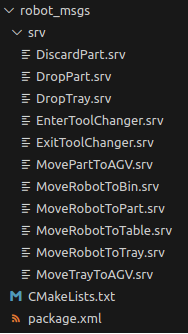
\includegraphics[scale=1]{images/custom_service_msgs.png}
    \caption{Custom Service Messages}
    \label{fig:cusSrvMsgs}
\end{figure}

\begin{figure}[h]
    \centering
    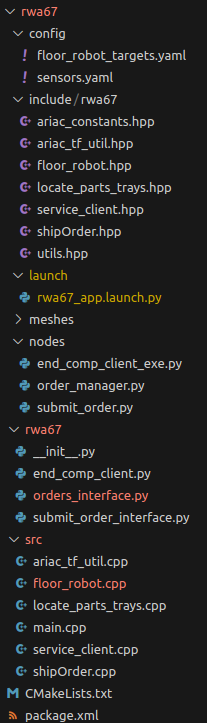
\includegraphics[scale=1]{images/main_competitor_package.png}
    \caption{Main Competitor Package}
    \label{fig:mnCompPkg}
\end{figure}

\clearpage
\justifying
\section{Environment Sensors}

\begin{figure}[h]
\centering
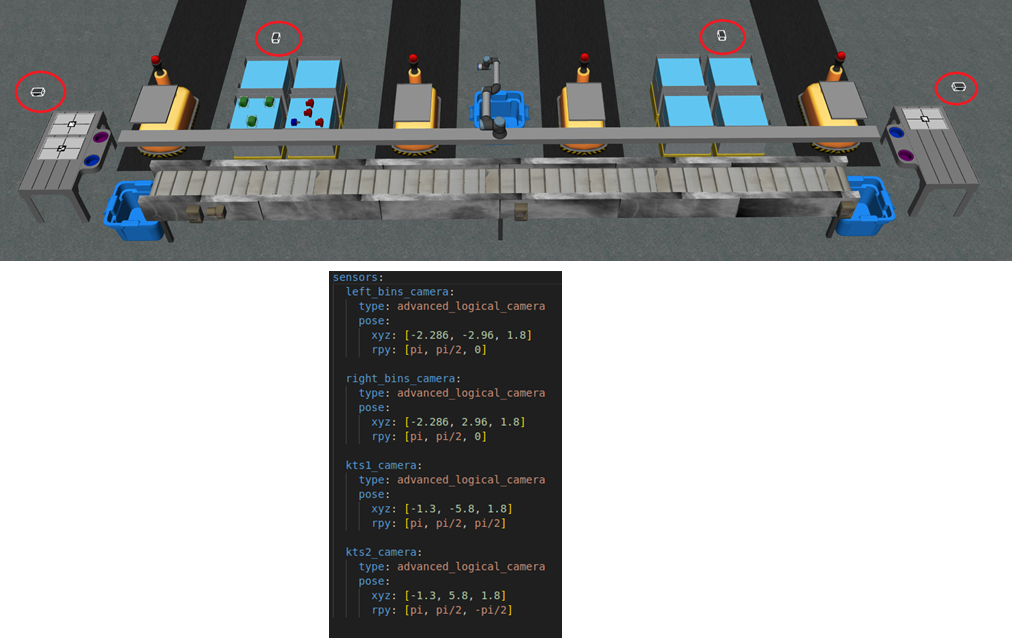
\includegraphics[scale=0.65]{images/environment_sensors.png}
\caption{Environment Sensors}
\label{fig:envSnsrs}
\end{figure}

The environmental sensors provide the CCS with information necessary to build the world model (part locations, tray locations). As highlighted with red circles, in the figure \ref{fig:envSnsrs}, the following are sensors deployed for the competition.

\begin{enumerate}
    \item \justifying 4x Advanced Logical Sensors
        \begin{enumerate}
            \item \justifying Provide tray id and pose
            \item \justifying Provide part pose, color, and type
        \end{enumerate}
    \item \justifying AGV Tray Sensors
        \begin{enumerate}
            \item \justifying Located on each AGV
            \item \justifying Provide quality information of tray and parts
        \end{enumerate}
\end{enumerate}

\justifying
\section{Order Manager} \label{OrderManager}
The Order Manager node is the heart of the competition package.
It monitors and controls the flow of order fulfilment. Based on the priority, the current order is executed until it is fulfilled. It interfaces with other different nodes including 'Locate parts and trays', 'ship order' and other nodes as shown in the block diagram.

The functionalities of the 'order manager' are depicted through following pseudo code:\\

\noindent \verb|Fullfill_order:|\\
	\verb|order = current_order|\\
	\verb|tray = order.tray|\\
	\verb|agv = order.agv|\\
	
	\noindent \verb|tray_pose = search_tray_inventory(tray)|\\
	\verb|move_robot_to_table()|\\
	\verb|change_to_tray_gripper()|\\
	\verb|grab_tray()|\\
	\verb|place_tray_on_agv()|\\
	\verb|remove_tray_from_inventory()|\\

	\noindent \verb|move_robot_to_table()|\\
	\verb|change_to_part_gripper()|\\
	\verb|for (part in list_of_parts):|\\
		\verb|part_pose = search_part_inventory(part)|\\
		\verb|    If (part_pose == None):|\\
			\verb|   Continue  #part not found… Moving on|\\
		\verb|    place_part_on_tray()|\\
		\verb|    perform_quality_check()|\\
		\verb|    If (faulty):|\\
			\verb|           Move part to bin|\\
			\verb|           Add part back to list_of_parts|\\\\


The order manager is subscribed to seven different topics, which can be grouped into three categories:\\
\noindent
\verb|/ariac/competition_state|\\ 
Begins fulfilling orders\\

\noindent
\verb|/ariac/orders|\\
Adds orders to the queues\\

\noindent
\verb|/left_bin_camera_data|\\
\verb|/right_bin_camera_data|\\
\verb|/kitting_tray1_camera_data|\\
\verb|/kitting_tray2_camera_data|\\
Records the poses of parts and trays. These have been obtained by \verb|locate_parts_trays|, translated to world pose, then republished.\\



\begin{figure}[h]
    \centering
    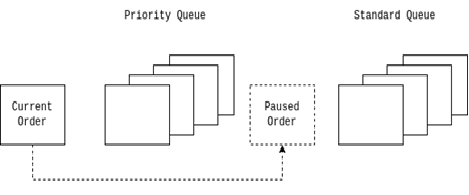
\includegraphics[scale=0.75]{images/queOrd.png}
    \caption{Order Queue}
    \label{fig:queOrd}
\end{figure}

\begin{figure}[h]
    \centering
    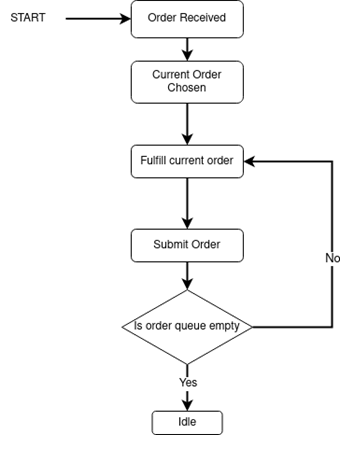
\includegraphics[scale=0.75]{images/order_manager.png}
    \caption{Order Manager}
    \label{fig:ordMgr}
\end{figure}



\justifying
\section{Trial Files}
\noindent Several trial files were developed to test the agility of the CCS. The purpose of these trial files is to create as many challenges in the competition as possible to observe whether the CCS is capable of handling these challenges without crashing. \\

\noindent The CCS was tested on the following trial files:\\
\begin{enumerate}
    \item \justifying \verb|rwa67summer2023.yaml|\\
        This trial file was provided as a part of RWA67.  The trial consists of 3 kitting orders, a faulty part challenge, and an insufficient part challenge.
    \item \justifying \verb|rwa67_summer2023_SB_test1.yaml|\\
        This trial file has 4 kitting orders with multiple faulty parts. Since the faulty parts are discarded the CCS also has to handle insufficient part challenge.\\
        The purpose of this trial file is to handle faulty and insufficient part challenges for multiple orders.\\
    \item \justifying \verb|rwa67_summer2023_TS_test1.yaml|\\
        This trial file has 5 similar parts in the environment for 1 kitting order. Out of 5 parts, 3 are faulty, hence, creating insufficient part challenge.\\
        The purpose of this trial file is to handle multiple faulty and insufficient part challenges in a single order.\\
 \end{enumerate}

\begin{figure}[h]
\centering
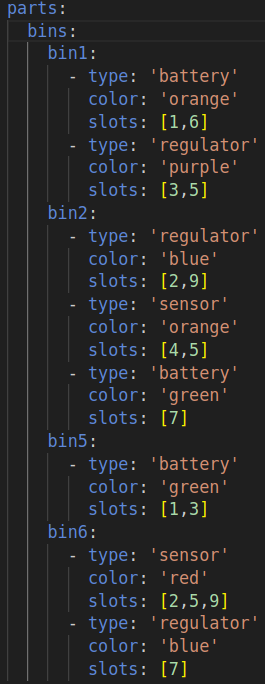
\includegraphics[scale=0.385]{images/rwa67_trial_1.png}
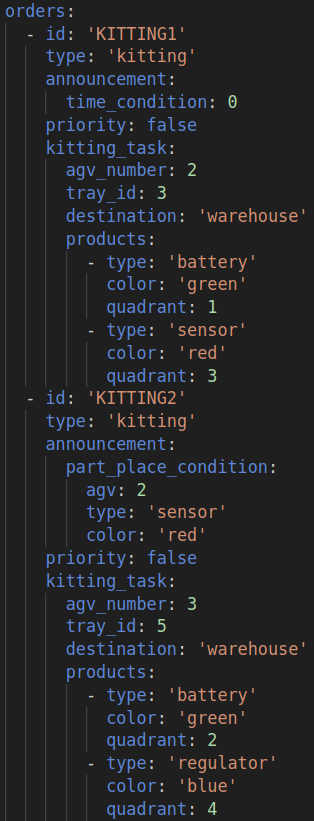
\includegraphics[scale=0.32]{images/rwa67_trial_3.png}
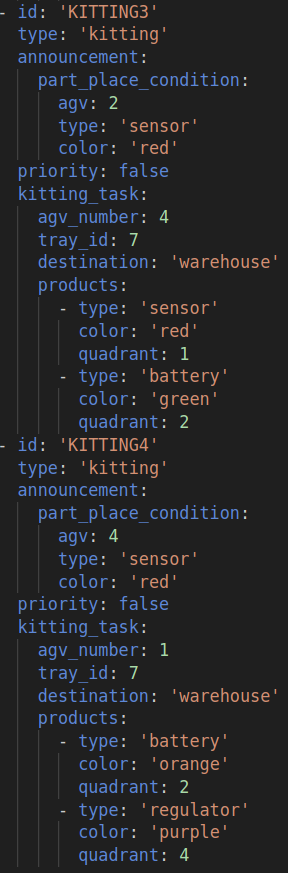
\includegraphics[scale=0.30]{images/rwa67_trial_4.png}
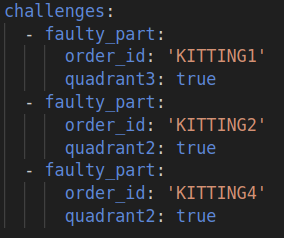
\includegraphics[scale=0.35]{images/rwa67_trial_5.png}
\caption{rwa67\_summer2023\_SB\_test1.yaml}
\label{fig:SBtest1}
\end{figure}

\begin{figure}[h]
\centering
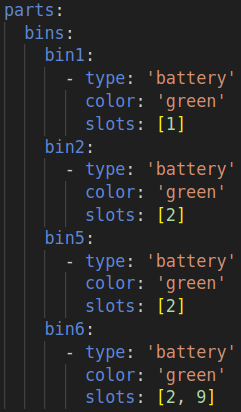
\includegraphics[scale=0.555]{images/rwa67_trial_6.png}
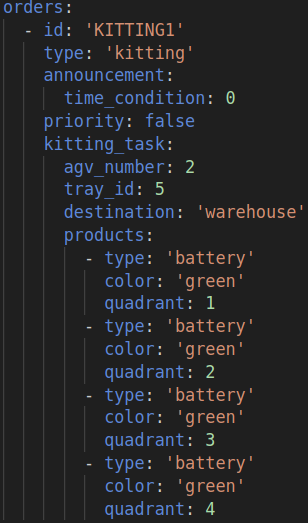
\includegraphics[scale=0.44]{images/rwa67_trial_7.png}
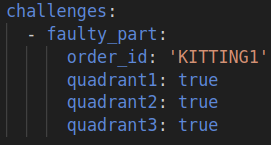
\includegraphics[scale=0.50]{images/rwa67_trial_8.png}
\caption{rwa67\_summer2023\_TS\_test1.yaml}
\label{fig:TStest1}
\end{figure}

\justifying
\section{Results}
The trial files were repeatedly used to check the robustness of trial file. Results of running above configuration files are as below:\\

\noindent \verb|rwa67_summer2023_SB_test1.yaml:|\\
completion time:  162 sec\\
Score: 39\\\\
\verb|rwa67_summer2023_TS_test1.yaml:|\\
completion time: 97 sec\\
Score: 9\\

\begin{figure}[h]
\centering
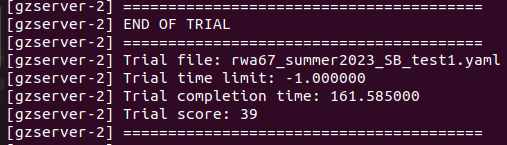
\includegraphics[scale=0.50]{images/rwa67_trial_11.png}
\caption{Result of rwa67\_summer2023\_SB\_test1.yaml}
\noindent ---\\
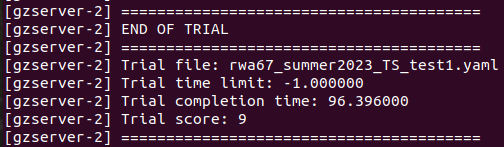
\includegraphics[scale=0.50]{images/rwa67_trial_12.png}
\caption{Result of rwa67\_summer2023\_TS\_test1.yaml}
\end{figure}

\noindent Scores and completion time for the both trial files remained similar throughout the testing cycle validating CCS designed to handle two different ARIAC challenges.

\justifying
\section{Difficulties Faced}
Numerous difficulties were faced to complete this RWA since it required a number of services for robot actions, moveit package to simulate robot movement in the gazebo environment, proper communication between services (written in C++) and clients (written in python) and many other programming challenges to create a robust CCS.\\ 
\noindent Below are some difficulties that were faced and the solutions to overcome them:\\
\begin{enumerate}
    \item Breaking down custom services:\\
    As the floor robot has to pick and place, both parts and trays - by changing gripper type, custom services had to be broken down for a smooth pick and place movement. To drop parts and trays on their new placed, two separate services were called and used - one before the part is dropped and another after the part is dropped. The purpose of breaking down the services here was to deactivate the gripper at a safe position to drop a part/tray.  

    \item Using appropriate moveit method to add collision objects in the environment:\\
    Using default addCollisionObject() method to add models in the planning scene was less useful when it came to detaching the object from the planning scene. Because of the nature of the method to run asynchronously, sometimes parts/trays were not added to the planning scene before they were dropped on their new placed. To avoid a crash in the program, when dropping a part/tray, applyCollisionObjects() method was used instead. This method made sure that the model was available in the planning scene right when the method itself was called.
    
    \item Adjusting waypoints:\\ 
    Waypoints in service callback methods used to pick up parts (move\_robot\_to\_part\_()) were updated with trial and error so that each type part didn't collide with other parts after being picked up from its place on a bin.  
\end{enumerate}

\justifying
\section{How can the results be made better?}
Due to the time constraints of the class, this CCS is not a completed CCS ready for competition in the ARIAC challenge.  CCS agility could be improved by:
\begin{enumerate}
    \item Tray and Part inventories are determined at start.  Ideally, part and tray locations should be continuously updated (bumped parts, dropped parts)
    \item Integrate ceiling robot to reach all parts in bins
    \item Attach trays/parts to AGVs in planning view.  Current implementation would cause collisions when using the AGV for a second time.
    \item Finish Priority order logic
    \item Create order logic for assembly stations
\end{enumerate}

\justifying
\section{Conclusion}
In summary, the project accomplishes its objectives of performing the motion planning to complete up to four orders (one per AGV), while demonstrating the ability to sufficiently handle insufficient parts and faulty parts.\\

\section{Contributions to the project}
\begin{itemize}
    \item Shreejay Badshah: Creating services and relevant servers, agility testing, fine-tuning moveit parameters.
    \item Arshad Shaik: Testing, launch files, presentation and LaTex report generation
    \item Tej Kiran: Code implementation - Qualitycheck, etc.
    \item Tim Sweeney: Worked on the logic of the Order Manager, the End Competition node, created test-trials
    \item Dhinesh Rajasekaran: Testing, documentation
    \item Ian Serbin: Code implementation - services, order manager
\end{itemize}

\justifying
\section{Acknowledgements}
We would like to thank Prof.Zeid Kootbally and Prof.Craig Schlenoff for their valuable guidance and feedback and their help in completing this project.
\section{Resources}
\begin{itemize}
    \item https://ros.org
    \item https://docs.ros.org/en/galactic/Tutorials.html
    \item https://stackoverflow.com
    \item https://www.nist.gov/el/intelligent-systems-division-73500/agile-robotics-industrial-automation-competition
    \item \verb|https://github.com/sbadshah96/ENPM663_RWA|
\end{itemize}

\printbibliography

\end{document}